\chapter{Filesystem Metaphore, Naming, and Verifiability}
From our experience with building applications, there are a clear set of requirements that are necessary.  Most applications
construct the notion of context using the naming convention ascribed to a sensor stream.  The name conflates the notion of system,
space, and type information.  At the very least, these three should be supported, however, often other categorical needs must be
met to perform various kinds of aggregate statistical, analytics, and control.  In addition, we need to support the management of
processing jobs that process stream data and provide integrated management facilities for them.

Building applications are essentially monitoring and control applications built on the streams generated by sensors embedded through
the building or distillates of them.  As the number of applications and streams increased, it becomes desireable to manage them 
in a centralized fashion.  Moreover, the centralized apporach allows all applications to make use of a uniform naming convention and
can allow applications to be interoperable.  Systems that wish to support such applications require the following properties:

\begin{enumerate}
\item Logically accessible physical resources.
\item Representation of data producing and data consuming elements.
\item Representation of inter-relationships between elements.
\item Provide uniform naming and access.
\end{enumerate}

This chapter describes the use of the filesystem and pipe abstraction for represents streams in space.  The filesystem naming convention
provide a a unified namespace to application, for accessing physical resources and streams.  Moreoever, we support multi-naming through
symbolic links -- an important requirement for building applications.  We also discuss the incorporation of a pipe-like mechanism for 
processing streams and their output.

\subsection{Introduction}
The United States leads the world in per-capita energy consumption.
Our electricity use has consistently increased over the last 40 years~\cite{oecd2011} and other parts of the world are rising all 
too rapidly.  With the specter of climate change and the increasing cost of energy, we must explore new
ways for individuals to gain visibility and insight into their energy consumption in order to optimize and reduce it. 
With the increasing penetration of embedded sensors in the environment and
the continued rise in smartphone adoption, we see an opportunity for smartphones to bridge the physical world
to our computational infrastructure and provide an `energy lens' on the physical world.  

We use mobile phones to construct an entity-relationship 
graph of the physical world and combine it with streaming sensor data in order to perform detailed energy-attribution.
We limit the scope of the world to a single building domain.  We have designed and implemented a real-time, mobile energy auditing
application, called the `Energy Lens', that allows us to collect information about 
things throughout the building and how they are related to each other.  For example, computer X is inside 
room Y and connected to meter Z.  Then, we use these relationships to guide our data look-up and analytical
calculations.  For example, the load curve of room Y consists of the sum of all the power traces for loads
inside room Y.  We use the mobile smartphone as the main input tool.  Our work examines \emph{three main challenges} in setting up and 
deploying a real, whole-building infrastructure to support real-time, 
fined grained energy analytics.  

The first challenge is related to tracking and mobility.
The use of mobile phones presents classical, fundamental challenges related to mobility.  Typically, mobility
refers to the phone, as the person carrying it moves from place to place.  However, in the energy-attribution
context, we are also referring to the movement of energy-consuming objects.  Tracking their relationships to spaces 
and people is as important as tracking people.  We describe how we deal with \emph{both moving people and 
moving objects} and show that these historically difficult problems can be addressed relatively easily, if the proper infrastructure is 
in place.  %We provide evidence that the approach is simple, incrementally deployable, and scalable.

The second challenge is about capturing the inter-relationship semantics and having these inform our  analytics.
We adopt the general notion of physical tags that identify objects in the world.  Our system uses \emph{QR codes} to tag things and locations 
in the physical world.  However, \emph{any tag that provides a unqiue identifier for an object could serve the same purpose}.
Once tagged, there are three types of interactions -- 
registration, linking, and scanning -- which establish important relationships.  Registration is the act of creating a virtual object 
to represent a physical one.  Linking captures the relationship between pairs of objects.  Scanning is the act of performing an item-lookup.
Each of these interactions requires a set of swiping gestures.  Linking requires two tag swipes while the other two actions
require a single tag swipe.  Internally, we maintain a \emph{entity-relationship graph (ERG)} of things, people, and locations, that gets
updated through these sets of gestures.

The third challenge is about indoor network connectivity and access.
In order to connect these components, we rely on having `ubiquitous' network connectivity.  However, in practice, network
\emph{availability} is intermittent and our system must deal with the challenges of intermittency.  We discuss how caching
and logging are used to address these challenges.  Moreover, when connectivity is re-established, we must deal with
applying updates to the ERG, as captured by the phone while disconnected.  
% Conflicts can also occur during an update.  For example, the two updates may disagree about which items are attached
% to which meters.  We implement a very simple conflict resolution scheme, described in section~\ref{sec:conflicts}.
% Finally, certain physical-state transitions are represented as a set of updates to the ERG that must be applied 
% atomically.  We implement transactions in the log-replay and transaction manager.
% Our `Energy Lens' system is deployed in a building on our campus.  We discuss
% its architecture and our design choices.  
  
% We also discuss novel strategies for tracking moving people/things and describe how we implement these in our system.  In summary, our work
% makes the following contributions:

% \begin{itemize}
% \item We design and implement a system that captures and combines physical entities, their inter-relationships, and real-time sensor data 
% 		in buildings.% using mobile phones, qr code, and a cloud-based infrastructure.
% \item We observe that certain combinations of swipes give us useful information to set the location of people and things over time.
% 		We codify this observation in our \emph{context-tracker} and use it to maintain consistency between the entity-relationship graph and the 
% 		state of the physical world.  To the best of our knowledge, this is radically different from the approaches in standard 
% 		localization techniques.  However, we argue that it can be used to \emph{enhance} their accuracy and overall performance.
% \item We implement a prefetching algorithm to obtain context-dependent information to both improve performance and
% 		enable disconnected operation.  We also design and implement a log-replay and transaction manager over our data management layer.  We describe how different conflict-resolution policies can be implemented and our rationale for the policies we chose.
% \end{itemize}

% \vspace{0.08in}

% In the next sections we go through a motivating scenario.  We then discuss some related work, followed 
% by the system architecture, evaluation, and future directions.



\section{Related Work}
HomeOs~\ref{homeos}


\section{File abstraction and Supporting Multiple Names}
Similar requirements to those aforementioned have been addressed in the design and implementation of filesystems.  Filesystems provide
logical access to physical resources through files, with different files and associated semantics, exposed to applications through a shell
or programmtically.  Filesystems representat collections of bits, encapsulated by a file, and grouped with folders.  Symbolic links support
the notion of multi-naming.  A single file or folder could have multiple names that lead to the same underlying object.  Filesystems even
support the notion of streaming data through character and block device files.  Moreover, pipe files allow programs to communite with each
other through a piece of shared memory, where the source application writes to the pipe and the sink application consumes from the pipe.

We assert that these constructs should be directly adopted for supporting applications in the buildings.  Our approach adopts the unix
file philosophy where everthing is represented as a file.  Each object created in StreamFS is assigned two names, by default, one which 
uniquely identifies the object and \emph{not} human-readable and the second which is changeable and human-readable.  Consider
the example shown in Figure~\cite{fig:everythingfile}.


\begin{figure}[t!] %htbp
\centering
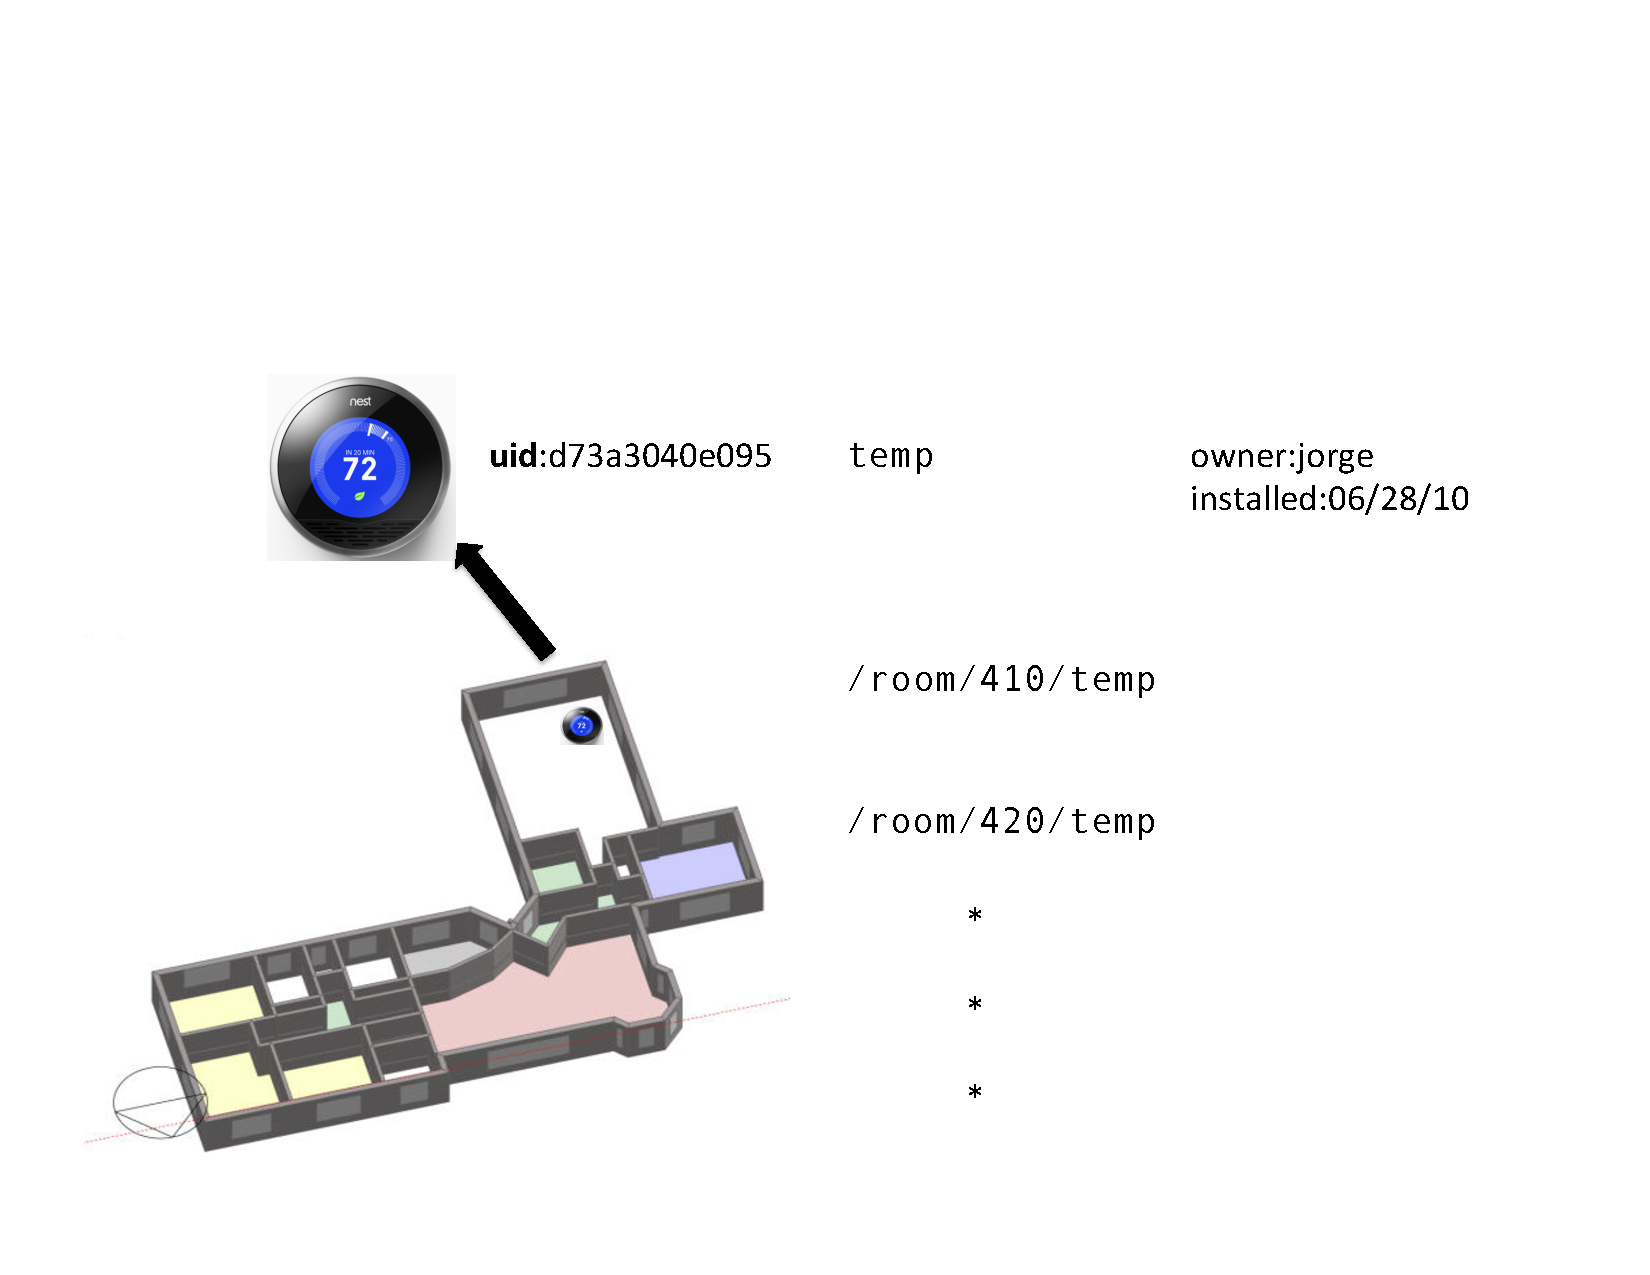
\includegraphics[width=0.65\columnwidth]{figs/everythingfile}
\caption{Everything is a file.  Temperature sensor represented as a file in a folder that contains folders for each room.
Note, the file that represents a temperature sensor producing a stream is given a unique identifer.  The user may also
decorate the file with extra metadata for searching purposes.}
\label{fig:everythingfile}
\end{figure}

In this example, the user is creating a temperature stream file in every room of the building.  The name of the file, given by the user,
is \emph{temp}.  Upon creation, the file is uniquely identified by the system using a unique identifier, as shown.  Like in a unix filesystem, the
file is created within a folder.  Ideally, the name of the folder would encode the placement of the sensor.  In the figure, the 
user is create a temperature stream file in room 410 and room 420.  Note the full filepath for the stream file is /room/410/temp.
During creation, the user may also decorate the file with extra metadata, also shown in the figure.  In this example, they have annotated
the file with information about the owner and when the sensor was installed.   This metadata is used for quickly locating the file
or grouping files that contain similar tags, quickly.

\subsection{File types and operations}
As we map the filesystem abstraction into this problem space, we need to consider the various kinds of files our system will contain,
their semantics, and how our system will expose and manage them.  There are essentially 4 types of files and 6 sub-types.  We summarize
these in Table~\ref{tab:filetypes}.  There are also different kinds of operations that the each file type supports.  Operational semantics
are file dependent.  For example, when you \emph{read} a folder, you obtain the metadata associated with the folder and the name
of its children.  When you \emph{read} a stream, you its metadata and the last timestamp-value it produced.  \emph{Writ}ing to a stream
is a bit different.  You can write to a stream to update its metadata tags and the stream source can write a value to it.  The stream
source is identified with a \emph{publish identifier} (pubid).  The stream source includes the pubid in the write operation for 
the specified stream file.  Without the pubid, the source cannot write to the file.  Any other writer should not be allowed to write to 
a stream file either.  

\begin{table}[h]
\begin{center}
\begin{tabular}{| r | l | l |}
	\hline
	\textbf{type} & \textbf{description} & \textbf{valid operations} \\ \hline
	default/folder & Container file.  Used to group other  & read, write, delete  \\
				   & kinds of files within it.  &  \\ \hline

	stream & Represents a data stream. & read, write, delete, subscribe, \\
			&							&query \\ \hline

	controller & Represents a controller. & read, write, subscribe \\ \hline

	special & There are several kinds of special files for  & read, delete \\
		    & management of jobs and pipes. &  \\ 
	\hline
\end{tabular}
\caption{Summary of the 4 main file types and their valid operations in StreamFS.}
\label{tab:filetypes}
\end{center}
\end{table}

Similar to a traditional filesystem, StreamFS includes \emph{special files}.  There are 6 special files and 5 of them 
are for management purposes.  The only one that is not is the \emph{symbolic link} file, which is essentially used to support
multi-naming and inherents the operational semantics of the file it points to.  The delete operation on a symlink, however,
only deletes the symlink.  A description of these files and the operations they support is given in Table~\ref{tab:filesubtypes}.
A detailed description and examples with be presented in later sections.


\begin{table}[h]
\begin{center}
\begin{tabular}{| r | l | l |}
	\hline
	\textbf{operation} & \textbf{file type} & \textbf{semantics} \\ \hline
	read & folder, stream, ipd, ipi, epd, epi, sub & read the metadata and tags for \\
		 &										   & the associated file. \\ \hline
	write &  stream & Write to stream file, only the \\ 
		  & 		& appropiate stream source is permitted.\\ \hline
	delete & folder, stream, ipd, ipi, epd, epi, sub & Folder must be empty.  \\
		   & 										 & The others can be directly deleted. \\ \hline
	query &  stream, all & streams support time-range queries.  \\
		  &			     & All support metadata-tag queries.\\ \hline
	subscribe & stream & Forwards data from a stream to the\\
			  &		   & specified destination.\\
	\hline
\end{tabular}
\caption{File opertaitons, the file types that support them, and their general semantics.}
\label{tab:semantics}
\end{center}
\end{table}

\subsubsection{Default, Stream, and Controller Files}


\subsubsection{Special Files}

\begin{table}[h]
\begin{center}
\begin{tabular}{| r | l | l |}
	\hline
	\textbf{type} & \textbf{description} & \textbf{valid operations} \\ \hline
	internal process defintion (ipd) & Javascript process definition.  & read, write, delete  \\ \hline

	internal process instance (ipi) & Management file used for managing & read, delete \\
							  & active processing of this script. & \\ \hline

	external process definition (epd) & Gives information about where an & read, write, delete \\
								& external process lives. &\\ \hline

	external process instance (epi) & An active processing stream to an  & read, write, delete \\
								& external process. &\\ \hline

	subscription instance (sub) & An instance of a subscription.  Contains & read, delete \\
								& information about the subscription, &\\
								& such as source/sink and related statistics &\\ \hline
	symbolic link (symlink) & Similar to a symbolic link in Unix. & \\
	\hline
\end{tabular}
\caption{Summary of the 6 special-file sub-types and their valid operations in StreamFS.}
\label{tab:filesubtypes}
\end{center}
\end{table}

\section{Verication through Sensor Data}

\section{Types of Verification}

\section{Summary}




